%=============================================================================
% INTRODUCTION
% This paper outlines the standard template for an MSci submission. In earlier years, MSci students at the School of Computing Science\endnote{\url{http://www.dcs.gla.ac.uk}}, University of Glasgow, were expected to produce a full-length dissertation. Now, the requirement is for MSci students to write a paper of up to 14 pages in length, using the supplied \texttt{mpaper} \LaTeX style file.

% The precise structure of an MSci paper is not mandated, but it should probably cover in detail the following aspects of the project.

% \begin{enumerate}
% \item General description of the problem, motivation, relevance
% \item Background information, possibly including a literature survey
% \item Description of approach taken to solve the problem, including high-level design and lower-level implementation details as appropriate
% \item Evaluation, qualitative or quantitative as appropriate
% \item Conclusion, including scope for future work
% \end{enumerate}

\documentclass[../mpaper.tex]{subfiles}
\begin{document}

There is significant importance given to a good User Experience in a product - which is reasonable - however, there is another area that requires equal importance which is Developer Experience; it pertains to the humans working on a project as software developers -- but project frustration is widespread in any industry. A person's mood affects their problem-solving skills and productivity \cite{amabileProgressPrincipleUsing2011,graziotinFeelingsMatterCorrelation2015,meyerSoftwareDevelopersPerceptions2014,mullerStuckFrustratedFlow2015}, and in software development, this influences performance on certain tasks such as implementing, testing and debugging \cite{khanMoodsAffectProgrammers2011}. Companies and organisations take measures on helping their staff destress and have a better experience, but this may not be effective or formalised. Software is different to other industries as it requires a level of mental cognition in unique, non-repeating processes \cite{trendowiczChapterFactorsInfluencing2009,abdel-hamidSlipperyPathProductivity1996,kemererEmpiricalValidationSoftware1987}. It must be realised that \textbf{humans are the most important aspect of software engineering \cite{martinAgileSoftwareDevelopment2003}}, and we plan to address the common obstacles and frustrations they face as they apply various disciplines to deliver reliable, efficient and high-quality products \cite{sommervilleSoftwareEngineering1992}.

User Experience (UX) involves all aspects of the interaction between \textbf{the end-user} \& the product representing the \textit{holistic} perspective of how a person feels using the system. There have been recognised heuristics outlined for interface design along with published articles in the International Organization for Standardization (ISO). ISO 9241\noteurl{https://www.iso.org/standard/77520.html} describes human-centered design as an approach to design systems that improve quality (of life) for users by 1) being comprehensive \& reducing training, 2) reducing discomfort and stress, 3) contributing towards sustainable objects without threatening life, and most importantly 4) \textbf{increasing the productivity and enhancing effectiveness \& efficiency of users and organisations} providing a competitive advantage.

Developer Experience (DX) is user experience from a developer's point-of-view, i.e. the user is a person involved in the process of software development, so the persona can be known to have relatively higher technical knowledge and the products they use are involved in the development process. It is part of a wider field called Developer Relations (DevRel) that focuses on managing relationships between organisations and developers; it can also be seen as part of marketing \& sales than engineering being similar to the field of Public Relations (PR). DevRel only started to become mainstream over the last decade with increasing SaaS startups like Twilio, Zendesk and Intuit.

In the same decade, access to fast internet, performant browsers \& mobile devices increased the demand for web development. PHP has been widely used to render HTML pages with CSS \& JavaScript, but with the introduction of JavaScript runtimes such as Node.js and Deno, developers could just use the knowledge for JavaScript for the server and client. Frameworks like Express, Webpack and Bootstrap also provided the base implementation of a server, renderer and component styling (respectively) for faster development; being open-source, they relied on referrals (compounding growth), rather than funding (linear) marketing, so they focused on providing great developer experience, support and documentation for good retention.

For example, modern languages like Rust and TypeScript became popular due to the development experience. Stack Overflow Developer Survey 2022\noteurl{https://survey.stackoverflow.co/2022/} reveals the most loved and most dreaded programming languages (see \autoref{fig:so_survey}); it also included a section on Developer Experience sharing that while more than 50\% had CI/CD \& DevOps functions, only 38\% had a developer portal (for tools and services) for their organisation and only 16\% had Innersource initiatives.

\begin{figure}
	\centering
    \resizebox{0.48\textwidth}{!}{%
	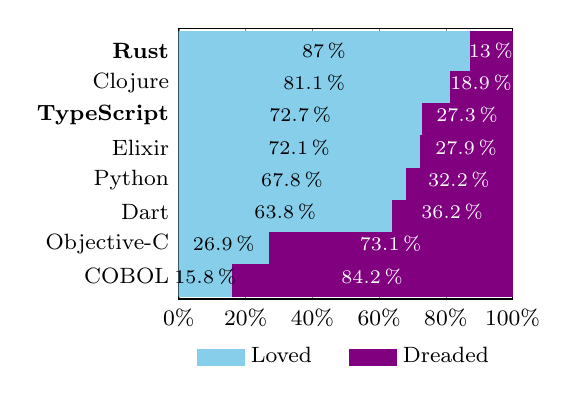
\begin{tikzpicture}
	\begin{axis}[
			xbar stacked,
			area legend,
			legend style={/tikz/every even column/.append style={column sep=0.4cm},at={(xticklabel cs:0.5)},anchor=north,legend columns=5,draw=none,font=\footnotesize},
			ytick=data,
			tick label style={font=\footnotesize},
			width=0.48\textwidth,
			xticklabel={\pgfmathparse{\tick}\pgfmathprintnumber{\pgfmathresult}\%},
			bar width=5mm,
			y dir=reverse,
			yticklabels={\textbf{Rust},Clojure,\textbf{TypeScript},Elixir,Python,Dart,Objective-C,COBOL},
			xmin=0, xmax=100,
            nodes near coords={\pgfkeys{/pgf/fpu}\pgfmathparse{\pgfplotspointmeta}\pgfmathprintnumber{\pgfmathresult}\,\%},
            nodes near coords style={font=\scriptsize, /pgf/number format/.cd,precision=1},
            % grid style={line width=.01pt},
		]
		% Loved
		\addplot[SkyBlue,fill=SkyBlue,text=black,
			postaction={
				% pattern=vertical lines
		}] coordinates {(86.98, 0)(81.12, 1)(72.73, 2)(72.11, 3)(67.83, 4)(63.77, 5)(26.93, 6)(15.79, 7)};

		% Dreaded
		\addplot[Purple,fill=Purple,text=white,
			postaction={
				% pattern=horizontal lines
		}] coordinates {(13.02, 0)(18.88, 1)(27.27, 2)(27.89, 3)(32.17, 4)(36.23, 5)(73.07, 6)(84.21, 7)};

		\legend{Loved,Dreaded}
	\end{axis}
	\end{tikzpicture}
     }
	\caption{Responses for programming languages}
    \label{fig:so_survey}
\end{figure}

The COVID-19 pandemic saw software being released and updated in faster sprints; for example, video conferencing was necessary over lockdown, and Zoom \& Microsoft Teams shipped with lots of bugs and minimum features that were fixed overtime with multiple releases. In such circumstances, companies aim to improve their resource allocation, process efficiency, and cost reduction, so they measure software productivity \cite{devanbuAnalyticalEmpiricalEvaluation1996} using automated metrics like source lines of code (SLOC) written \cite{walstonMethodProgrammingMeasurement1977,devanbuAnalyticalEmpiricalEvaluation1996}, function points \cite{albrecht1979measuring,computerstaffSoftwareMetricsGood1994}, changes request fulfilled \cite{cataldoSociotechnicalCongruenceFramework2008,millerHowWasYour2021}, and vague \textit{timesheets}; these are highly objective \& inaccurate at capturing a developer's efforts. There could be a lot of effort put to make a commit of 3 additions and 2 deletions, and development should acknowledge it so future resources aren't wasted. Ensuring good productivity in a process ensures good development experience \cite{amabileProgressPrincipleUsing2011,graziotinFeelingsMatterCorrelation2015,meyerSoftwareDevelopersPerceptions2014,mullerStuckFrustratedFlow2015}. It is essential to recognise that developers are humans\noteurl{https://twitter.com/mahemoff/status/1947230411948032} and to include the hidden fourth-corner of The Project Management Triangle (Barners, 1980) which is "\textit{Emotional Cost}" (see \autoref{fig:management_triangle}).

\begin{figure}
    \centering
    \begin{subfigure}{0.22\textwidth}
        \resizebox{\textwidth}{!}{%
        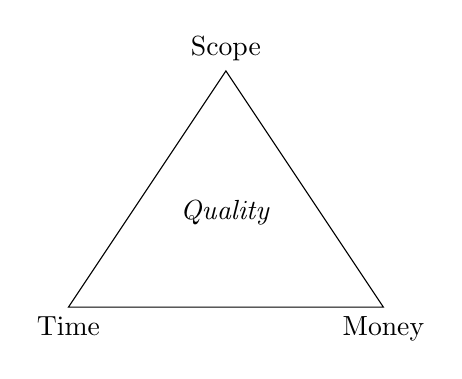
\begin{tikzpicture}
        \draw (0,0) node[anchor=north]{Time}
          -- (4,0) node[anchor=north]{Money}
          -- (2,3) node[anchor=south]{Scope}
          -- cycle;
        
        \draw (2,1.2) node{\textit{Quality}};
        \end{tikzpicture}
        }
    \end{subfigure}
    \hfill
    \begin{subfigure}{0.23\textwidth}
        \resizebox{\textwidth}{!}{%
        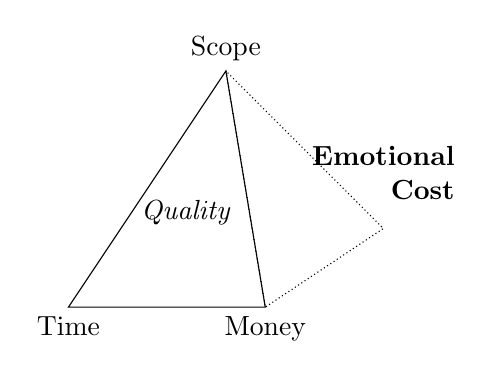
\begin{tikzpicture}
        \draw (0,0) node[anchor=north]{Time}
          -- (2.5,0) node[anchor=north]{Money}
          -- (2,3) node[anchor=south]{Scope}
          -- cycle;
        \draw (1.5,1.2) node{\textit{Quality}};
        \draw[densely dotted] (2,3) node[anchor=south]{}
          -- (2.5,0) node[anchor=north]{}
          -- (4,1) node[
                anchor=south,
                % text width=2cm,
                label={[align=right, font=\bfseries]{Emotional\\Cost}}
                ]{}
                % ]{\textbf{Emotional\\Cost}}
          -- cycle;
        \end{tikzpicture}
        }
    \end{subfigure}
    \caption{Project Management Triangle}
    \label{fig:management_triangle}
\end{figure}

\vskip8pt \noindent {\bf Contributions.} In this paper, we present the design and implementation of a dashboard that explicitly links developer experience with their productivity through the activity between the discrete commit events integrating data from sources and structuring it to produce new metrics that give a comprehensive insight into development effort so that task-estimations can be more accurate and developers increase productivity therefore improving their developer experience.

\vskip4pt \noindent All information about the project can be found on\\\url{https://github.com/ineshbose/code-fitness}.

\vskip6pt \noindent
{\bf This paper is structured as follows.}
% In \autoref{sec:Background}, we provide an overview and background on the concept of Developer Experience (DX), discussing its importance and relevance in software development.
\autoref{sec:RelatedWork} describes previous work in related areas, highlighting the gaps and limitations of existing solutions.
\autoref{sec:Design} presents our proposed solution and its design, explaining how it addresses the outlined issues.
In \autoref{sec:Implementation}, we describe the implementation details, including the tools and technologies used to develop the solution.
\autoref{sec:Evaluation} shares the evaluation methodology and results for our experiment, with feedback received from the users, showing how the solution performed in terms of usability, performance, and user satisfaction.
\autoref{sec:Conclusion} concludes the paper by summarising the key findings and contributions with potential future work that can build on this research to further enhance developer experience.

\end{document}
